\documentclass[10pt,pdf,aspectratio=169]{beamer}

\usefonttheme[onlymath]{serif}
\usepackage{amsmath,amsfonts,amssymb,amsthm,mathtools}
\usepackage[T2A]{fontenc}
\usepackage[utf8]{inputenc}
\usepackage[english,ukrainian]{babel}
\usepackage{ragged2e}
\justifying
\addtobeamertemplate{navigation symbols}{}{%
    \usebeamerfont{footline}%
    \usebeamercolor[fg]{footline}%
    \hspace{1em}%
    \insertframenumber/\inserttotalframenumber
}

\usepackage{tikz}
\usepackage{pgfplots}
\usepgfplotslibrary{fillbetween}
\pgfplotsset{compat=1.17}

\usetikzlibrary{patterns}
\usetikzlibrary{shapes.geometric}
\usetikzlibrary{arrows.meta}
\usetikzlibrary{shapes.geometric}
\usetikzlibrary{positioning,arrows}
\usetikzlibrary{decorations.markings}
\usetikzlibrary{calc}
\tikzset{
	block/.style={
		draw, 
		rectangle, 
		minimum height=1cm, 
		minimum width=3cm, align=center
	}, 
	line/.style={->,>=stealth'}}
\tikzset{>=latex}

\newcommand\centerarc{} % just for safety
\def\centerarc[#1]#2(#3)#4(#5:#6:#7)% [draw options] (center) (initial angle:final angle:radius)
  {\draw[#1]($(#3)+({#7*cos(#5)},{#7*sin(#5)})$)arc(#5:#6:#7);}

\newcommand{\R}{\mathbb{R}}
\newcommand{\vf}{\varphi}
\renewcommand{\d}[1]{\dot{#1}}
\newcommand{\dd}[1]{\ddot{#1}}
\newcommand{\E}{\mathcal{E}}
\newcommand{\T}{\mathcal{T}}
\newcommand{\bvec}[1]{\boldsymbol{\rm #1}}
\renewcommand{\l}{\left}
\renewcommand{\r}{\right}
\newcommand{\norm}[1]{\left\Vert #1 \right\Vert}
\newcommand{\intl}{\int\limits}
\newcommand{\suml}{\sum\limits}
\newcommand{\dotprod}[2]{\l< #1, #2\r>}
\newcommand{\Lap}[1]{\mathcal{L}\l\{#1\r\}}
\newcommand{\LapInv}[1]{\mathcal{L}^{-1}\l\{#1\r\}}
\def\setdif{\mathbin{\ooalign{\hss\raise1ex\hbox{.}\hss\cr
  \mathsurround=0pt$-$}}}

\usepackage{graphicx}
\graphicspath{ {./pics/} }

\usetheme{Luebeck}
\title{Основи диференціальних ігор}
\author{О. Галганов, Н. Фордуй}


\date{}
\begin{document}
    \begin{frame}
        \titlepage
    \end{frame}
    \begin{frame}
        \frametitle{Історія виникнення}
        Класична теорія ігор, творцями якої є Джон фон Нейман та Оскар Морґенштерн,
        оперує матричними іграми та зв'язаними з ними поняттями. Такі ігри зовсім не покривають всі можливості формалізувати процеси,
        в яких гравці приймають рішення. Наприклад, якщо розглядати задачу про оптимальну траєкторію руху
        корабля від керованої торпеди, яка його переслідує, то необхідно досліджувати не просто скінченний набір можливих дій
        кожного з гравців, а континуум можливих стратегій, кожна з яких відповідає деякій комбінації траєкторій руху корабля та торпеди.

        Сам термін <<диференціальна гра>> було введено Руфусом Айзексом --- одним з основоположників теорії диференціальних ігор.
    \end{frame}
    \begin{frame}
        \frametitle{Історія виникнення}
        \begin{tabular}{c c c}
            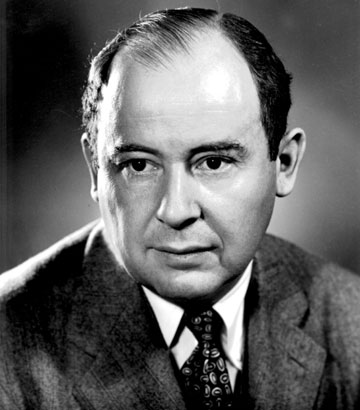
\includegraphics[scale=0.275]{../pics/John_von_Neumann.jpg} &
            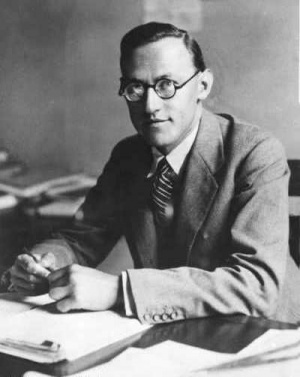
\includegraphics[scale=0.4]{../pics/Oskar_Morgenstern.jpg} &
            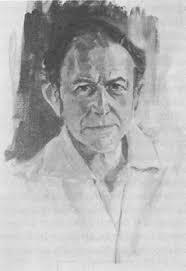
\includegraphics[scale=0.42]{../pics/Rufus_Isaacs.jpg} \\
            Джон фон Нейман &
            Оскар Морґенштерн &
            Руфус Айзекс
        \end{tabular}
    \end{frame}
    \begin{frame}
        \frametitle{Основні поняття}
    
        Рiшення, що їх приймають гравцi, полягають у виборi так званих \textbf{керувань}, вiд яких залежать \textbf{фазовi координати}: 
        їх значення у будь-який момент часу повнiстю визначає хiд гри, характеризуючи положення гравцiв у деякому просторi — \textbf{фазовому просторi}. 

        Поточнi значення фазових координат завжди вiдомi
        гравцям — тобто, це iгри з повною iнформацiєю. Невiдомим зазвичай є
        характер їх змiни: тобто, \textbf{керування} фазовими змiнними гравцями.
        \begin{block}{Приклад}
            Положення матеріальної точки на площині описується двома координатами $x_1$ та $x_2$. 
            Нехай швидкість руху точки є сталою $v$, а гравець обирає напрямок швидкості $\vf$ та може змінювати його у будь-який момент часу --- тобто, $\vf$
            є керуванням. Тоді рух точки описується системою диференціальних рівнянь
            \begin{gather*}
                \begin{cases}
                    \d{x_1} = v \cos \vf \\
                    \d{x_2} = v \sin \vf
                \end{cases}
            \end{gather*}
        \end{block}
    \end{frame}
    \begin{frame}
        \frametitle{Приклад}
    
        Геометричне положення автомобіля на декартовій площині описується трьома фазовими координатами:
        $x_1, x_2$ --- положення деякої точки автомобіля, $x_3$ --- кут, який утворює вісь вздовж автомобіля
        з деяким фіксованим напрямком --- наприклад, $x_1$.
        \begin{center}
            \begin{tikzpicture}
                \draw [->, thick] (-0.5, 0) -- (5, 0);
                \draw [->, thick] (0, -0.5) -- (0, 3);
                \node [below] at (5, 0) {$x_1$};
                \node [left] at (0, 3) {$x_2$};
                \filldraw [fill=lightgray, rounded corners, rotate around={-40:(1,1)}] (1, 1) rectangle (1.7, 2.4);
                \fill [rotate around={-40:(1,1)}] (1.35, 2.4) circle [radius=2pt];
                \draw [->, dashed, rotate around={-40:(1,1)}] (1.35, 0) -- (1.35, 3);
                \draw (0.83, 0) arc (0:44:0.2);
                \draw (0.93, 0) arc (0:45:0.3);
                \node [right] at (0.9, 0.22) {$x_3$};
            \end{tikzpicture}
        \end{center}
    \end{frame}
    \begin{frame}
        \frametitle{Продовження приклада}

        Нехай $A$ --- максимальне можливе прискорення автомобіля, тоді прискорення може набувати значень
        $A \vf_1$, де $\vf_1 \in [0; 1]$ і знаходиться під контролем гравця-водія. Можна ввести ще одну фазову координату $x_4$ --- швидкість автомобіля.
        Як ще одну фазову координату $x_5$ можна ввести кривину
        (фізично --- це кут повороту передніх коліс), керуванням якої є $W \vf_2$, де $\vf_2 \in [-1; 1]$, а $W$ --- максимальна швидкість зміни $x_5$.

        Система задає рух автомобіля у деякій диференціальній грі:
        \begin{gather*}
            \begin{cases}
                \d{x_1} = x_4 \cos{x_3} \\
                \d{x_2} = x_4 \sin{x_3} \\
                \d{x_3} = x_4 x_5 \\
                \d{x_4} = A \vf_1, \; \vf_1 \in [0; 1] \\
                \d{x_5} = W \vf_2, \; \vf_2 \in [-1; 1]
            \end{cases}
        \end{gather*}
    \end{frame}
    \begin{frame}
        \frametitle{Опис руху}
    
        Вважаємо, що гра відбувається у \emph{фазовому просторі} $\E$ --- деякій області в $\R^n$ та на її межі.
        Рух точки $x = \l(x_1, x_2, ..., x_n \r)$ у фазовому просторі описується системою диференціальних рівнянь
        \begin{gather*}\label{eq_1}
            \begin{cases}
                \d{x_1}(t) = f_1(x_1(t), ..., x_n(t), u_1(x, t), ..., u_P(x, t), v_1(x, t), ..., w_E(x, t)) \\
                \d{x_2}(t) = f_2(x_1(t), ..., x_n(t), u_1(x, t), ..., u_P(x, t), v_1(x, t), ..., w_E(x, t)) \\
                \dots \\
                \d{x_n}(t) = f_n(x_1(t), ..., x_n(t), u_1(x, t), ..., u_P(x, t), v_1(x, t), ..., w_E(x, t)) \\
                x_1(0) = x_1^0, x_2(0) = x_2^0, ..., x_n(0) = x_n^0
            \end{cases}
        \end{gather*}
        або, коротше,
        \begin{gather*}\label{eq_2}
            \begin{cases}
                \d{x}(t) = {f}(x(t), u(x, t), v(x, t)) \\
                x(0) = x_0
            \end{cases}
        \end{gather*}
        Ці рівняння називаються \emph{рівняннями руху}. Функції $f_j$ є заданими та вважаються достатньо гладкими.
    \end{frame}
    \begin{frame}
        \frametitle{Приклад (гра <<водій-вбивця>>)}
    
        Гра відбувається на площині. Переслідувач $P$ рухається зі сталою швидкістю $w_P$, радіус кривини його траєкторії обмежений
        заданою величиною $R$. Керування $P$ --- це вибір значення кривини в кожний момент часу. Рух утікача $E$ простий: швидкість $w_E$ фіксована,
        керуванням є вибір напрямку швидкості $v(t)$. $E$ є більш маневреним, ніж $P$.
        Фазовими координатами в цій грі є пари $x_P, y_P$ і $x_E, y_E$ для опису положення $P$ та $E$ відповідно, та $\theta$ --- напрямок руху $P$.
        \begin{center}
            \begin{tikzpicture}[scale=0.75]
                \draw [->, thick] (-0.5, 0) -- (7, 0);
                \draw [->, thick] (0, -0.5) -- (0, 5);
                \node [below] at (7, 0) {$x$};
                \node [left] at (0, 5) {$y$};
                % P
                \fill (1.5, 2) circle [radius=2pt];
                \node [below left] at (1.5, 2) {$P$};
                \draw [dashed] (1.5, 2) -- (1.5, 0);
                \draw [dashed] (1.5, 2) -- (0, 2);
                \node [below] at (1.5, 0) {$x_P$};
                \node [left] at (0, 2) {$y_P$};
                \draw (1.5, 2) -- (1.5, 2.7);
                \draw [thick, ->, rotate around={-50:(1.5, 2)}] (1.5, 2) -- (1.5, 3);
                \centerarc[] (1.5, 2) (40:90:0.5);
                \node [above right] at (1.5+0.05, 2+0.35) {$\theta$};
                \draw [thick, rotate around={-50:(1.5, 2)}] (1.5-3, 2) -- (1.5+3.5, 2);
                \fill [rotate around={-50:(1.5, 2)}] (1.5-1.5, 2) circle [radius=2pt];
                \node [below] at (0.4, 3.1) {$C'$};
                \fill [rotate around={-50:(1.5, 2)}] (1.5+1.5, 2) circle [radius=2pt];
                \node [above] at (2.76, 0.71) {$C$};
                \fill [rotate around={-50:(1.5, 2)}] (1.5+2.2, 2) circle [radius=2pt];
                \node [above] at (3.3, 0.1) {$C_1$};
                % E
                \fill (5, 3.5) circle [radius=2pt];
                \node [below left] at (5, 3.5) {$E$};
                \draw [dashed] (5, 3.5) -- (5, 0);
                \draw [dashed] (5, 3.5) -- (0, 3.5);
                \node [below] at (5, 0) {$x_E$};
                \node [left] at (0, 3.5) {$y_E$};
                \draw (5, 3.5) -- (5, 4.2);
                \draw [thick, ->, rotate around={-60:(5, 3.5)}] (5, 3.5) -- (5, 4.5);
                \centerarc[] (5, 3.5) (30:90:0.5);
                \node [above right] at (5+0.05, 3.5+0.35) {$v$};
            \end{tikzpicture}
        \end{center}
    \end{frame}
    \begin{frame}
        \frametitle{Приклад (гра <<водій-вбивця>>)}
        Керування $E$ --- це вибір кута швидкості $v$. Керування $P$ записати дещо складніше. Проведемо через точку $(x_P, y_P)$
        пряму $C' P C$, $|C' P| = |P C| = R$, перпендикулярну до вектору швидкості $P$. $P$ обирає миттєвий центр кривини своєї траєкторії у довільній точці $C_1$ цієї
        прямої, що лежить за межами відрізку $C' C$ (оскільки радіус кривини обмежений). Керування $u(t)$ будемо вважати рівним за модулем
        $R / |P C_1|$, додатним для точок $C_1$, що знаходяться правіше від $P$, та від'ємним для тих, що знаходяться лівіше. Остаточно, маємо такі рівняння руху:
        \begin{gather*}
            \begin{cases}
                \d{x_P}(t) = w_P \sin \theta(t) \\
                \d{y_P}(t) = w_P \cos \theta(t) \\
                \d{x_E}(t) = w_E \sin v(t) \\
                \d{y_E}(t) = w_E \cos v(t) \\
                \d{\theta}(t) = \frac{w_P}{R} u(t), \; u(t) \in [-1; 1]
            \end{cases}
        \end{gather*}
    \end{frame}
    \begin{frame}
        \frametitle{Виграші}
    
        Мета диференціальної гри визначається виграшем, який залежить від траєкторій гравців. 
        Позначимо ці траєкторії як функції від часу як $x(t)$ та $y(t)$. 
        Зауважимо, що диференціальні ігри є \emph{антагоністичними} (або ж, \emph{іграми з нульовою сумою}).

        Якщо гра триває деякий заздалегідь визначений час $T$, то виграш гравця $E$ визначається
        як $H(x(t), y(T))$, де $H : \R^n \times \R^n \to \R$ --- деяка функція (нагадаємо, що розмірність $\E$ --- $n$).

        \begin{block}{Приклади виграшів}
            \begin{enumerate}
                \item $H(x(T), y(T)) = \norm{x(T) - y(T)}$
                \item $H(x(T), y(T)) = \underset{0 \leq t \leq T}{\min} \norm{x(t) - y(t)}$
                \item $H(x(T), y(T)) = t_* = \min \l\{ t \geq 0 : (x(t), y(t)) \in \T\r\}$
            \end{enumerate}
        \end{block}
    \end{frame}
    \begin{frame}
        \frametitle{Приклад}
    
        Розглянемо переслідування на площині з простим рухом, що описується системою
        \begin{gather*}
            \begin{cases}
                \d{x_1} = u_1, \d{x_2} = u_2, \; u_1^2 + u_2^2 \leq \alpha^2 \\
                \d{y_1} = v_1, \d{y_2} = v_2, \; v_1^2 + v_2^2 \leq \beta^2 \\
                x_1(0) = x_1^0, x_2(0) = x_2^0, y_1(0) = y_1^0, y_2(0) = y_2^0
            \end{cases}
        \end{gather*}

        Якщо $\alpha > \beta$, то гравець $P$ може гарантувати
        \begin{gather*}
            \forall l \geq 0 : \min \l\{ t \geq 0 : \norm{P(t) - E(t)} \leq l\r\} < +\infty
        \end{gather*}

        Якщо $\alpha \leq \beta$, то в разі $\norm{P(0) - E(0)} > l$ для всіх $l \geq 0$ гравець $E$, рухаючись від $P$ по прямій з максимальною швидкістю,
        зможе уникнути захоплення гравцем $P$.
    \end{frame}
    \begin{frame}
        \frametitle{Поняття стратегії}
    
        \begin{block}{Означення}
            \emph{Стратегіями} у диференціальній грі є вибір керувань $u$ та $v$ як функцій від часу $t$ та
            фазових координат $x$ у системі рівнянь руху
            $$
            \begin{cases}
                \d{x}(t) = {f}(x(t), u(x, t), v(x, t)) \\
                x(0) = x_0
            \end{cases}
            $$
        \end{block}
        Керування вважаються кусково-гладкими як компроміс між забезпеченням існування розв'язку, 
        (його може не існувати у класі неперервних функцій) та його єдиності (вона може порушуватися, якщо не вимагати неперервності розв'язку).

        Позначатимемо через $\rm P$ та $\rm E$ множини кусково-неперервних стратегій (керувань) гравців $P$ та $E$. 
    \end{frame}
    \begin{frame}
        \frametitle{Ситуація}
    
        Надалі для спрощення розглядатимемо не один вектор $x$, а два вектори $x$ та $y$, що відповідатимуть руху кожного з гравців. Тоді
        систему можна записати як
        \begin{gather*}
            \begin{cases}
                \d{x}(t) = f(x(t), u(x, y, t)) \\
                \d{y}(t) = g(x(t), v(x, y, t)) \\
                x(0) = x_0, y(0) = y_0
            \end{cases}
        \end{gather*}

        \begin{block}{Означення}
            Набір $S = \l\{x_0, y_0, u(\cdot), v(\cdot) \r\}$, де $x_0, y_0$ --- початкові умови, а $u \in \rm P$, $v \in \rm E$ --- керування, 
            називається \emph{ситуацією} в диференціальній грі.
        \end{block}

        
    \end{frame}
    \begin{frame}
        \frametitle{Умова існування та єдиності траекторій}
    
        Якщо розглядати траєкторії, що залежать лише від часу $t$ та накладати на $f$ та $g$ умови
        обмеженості та ліпшицевості по $x$ та $y$, тобто
        \begin{gather*}
            \norm{f(x_1, u) - f(x_2, u)} \leq \alpha \cdot \norm{x_1 - x_2}, \\
            \norm{g(y_1, v) - g(y_2, v)} \leq \beta \cdot \norm{y_1 - y_2},
        \end{gather*}
        то за теоремою про існування та єдиність роз'язку задачі Коші, для кожної ситуації $S$ буде існувати єдина пара траєкторій $x(t), y(t)$,
        для якої 
        \begin{gather*}
            \begin{cases}
                \d{x}(t) = f(x(t), u(t)) \\
                \d{y}(t) = g(y(t), v(t)) \\
                x(0) = x_0, y(0) = y_0
            \end{cases}
        \end{gather*}
    \end{frame}
    \begin{frame}
        \frametitle{Формальне визначення виграшів та їх види}

        \begin{block}{Означення}
            Користуючись означенням ситуації, можна ввести \emph{виграш} в ситуації $S = \l\{x_0, y_0, u(\cdot), v(\cdot) \r\}$
            як функцію $K(x_0, y_0, u(\cdot), v(\cdot))$.
        \end{block}

        Наведемо строгі означення чотирьох видів виграшів.

        \begin{block}{Означення}
            \begin{enumerate}
                \item \emph{Термінальний виграш.} Задано деяке число $t>0$ та неперервна по $x$ та $y$ функція $H(x, y)$. Виграш в ситуації $\l\{x_0, y_0, u(\cdot), v(\cdot) \r\}$
                визначається як:
                \begin{gather*}
                    K(x_0, y_0, u(\cdot), v(\cdot)) = H(x(T), y(T))
                \end{gather*}
            \end{enumerate}
        \end{block}
    \end{frame}
    \begin{frame}
        \frametitle{Види виграшів}
        
        \begin{block}{Означення}
            \begin{enumerate}
                \setcounter{enumi}{1}
                \item \emph{Мінімальний результат}. Задано деяке число $t>0$ та неперервна по $x$ та $y$ функція $H(x, y)$. Виграш в ситуації $\l\{x_0, y_0, u(\cdot), v(\cdot) \r\}$
                визначається як
                \begin{gather*}
                    K(x_0, y_0, u(\cdot), v(\cdot)) = \underset{0 \leq t \leq T}{\min} H(x(t), y(t))
                \end{gather*}

                \item  \emph{Інтегральний виграш}. Нехай $\T$ --- деяка підмножина $\R^n \times \R^n$, $H(x, y)$ --- неперервна функція. Нехай в ситуації $\l\{x_0, y_0, u(\cdot), v(\cdot) \r\}$
                $t_*$ --- перший момент потрапляння траєкторії $(x(t), y(t))$ на $\T$.
                Тоді
                \begin{gather*}
                    K(x_0, y_0, u(\cdot), v(\cdot)) = \intl_0^{t_*} H(x(t), y(t)) dt
                \end{gather*}
                де при $t_* = +\infty$ покладається $K = +\infty$.

            \end{enumerate}
        \end{block}
    
    \end{frame}
    \begin{frame}
        \frametitle{Види виграшів}
    
        \begin{block}{Означення}
            \begin{enumerate}
                \setcounter{enumi}{3}
                \item \emph{Якісний виграш}. Нехай $\T$ та $\mathcal{L}$ --- деякі підмножини $\R^n \times \R^n$, а $t_*$ --- перший момент потрапляння траєкторії $(x(t), y(t))$ на $\T$
                в ситуації $\l\{x_0, y_0, u(\cdot), v(\cdot) \r\}$. Тоді
                \begin{gather*}
                    K(x_0, y_0, u(\cdot), v(\cdot)) = \begin{cases}
                        1, & \text{ якщо } (x(t_*), y(t_*)) \in \mathcal{L} \\
                        0, & \text{ якщо } t_* = +\infty \\
                        -1, & \text{ якщо } (x(t_*), y(t_*)) \notin \mathcal{L} \\
                    \end{cases}
                \end{gather*}
            \end{enumerate}
        \end{block}
    \end{frame}
    \begin{frame}
        \frametitle{Нормальна форма диференціальної гри}
    
        Нарешті, можна дати означення нормальної форми диференціальної гри.

        \begin{block}{Означення}
            Нормальною формою диференціальної гри $\Gamma (x_0, y_0)$, заданої на просторі стратегій $\mathrm{P} \times \mathrm{E}$, називається система
            \begin{gather*}
                \Gamma (x_0, y_0) = \l<x_0, y_0, \mathrm {P}, \mathrm{E}, K(x_0, y_0, u(\cdot), v(\cdot)) \r>
            \end{gather*}
            де $K(x_0, y_0, u(\cdot), v(\cdot))$ --- функція виграшу, визначена будь-який з чотирьох способів вище.
        \end{block}

        Кожній парі $(x_0, y_0) \in \R^n \times \R^n$ відповідає своя гра в нормальній формі, тобто, фактично,
        визначається двопараметрична сім'я ігор, що залежать від $(x_0, y_0)$.
    \end{frame}
    \begin{frame}
        \frametitle{Простий рух на площині}
    
        Розглянемо найпростіші моделі задач переслідування --- диференціальні ігри на площині з двома учасниками:
        переслідувачем $P$ та утікачем $E$, траєкторії яких відповідно позначатимемо $x(t)$ та $y(t)$.
        Під \emph{простим рухом} мається на увазі, що закони їх руху описуються системою
        \begin{gather*}
            \begin{cases}
                \d{x} = u, & \norm{u} \leq \alpha \\
                \d{y} = v, & \norm{v} \leq \beta 
            \end{cases}
        \end{gather*}
        Тут $\norm{z} = \sqrt{z_1^2 + z_2^2}$.
        Такі закони руху означають, що гравці рухаються з обмеженою швидкістю,
        але напрямок руху можуть змінювати довільно. Проінтегрувавши рівняння, можна явно записати траєкторії руху як
        \begin{gather*}
            x(t) = x(0) + \intl_0^t u(s) ds, \;
            y(t) = y(0) + \intl_0^t v(s) ds
        \end{gather*}
    \end{frame}
    \begin{frame}
        \frametitle{Приклад}
        \begin{block}{Умова}
            Нехай $u(t) = \begin{pmatrix} -\sin t \\ 2 \cos {2t}\end{pmatrix}$, 
            $v(t) = \begin{pmatrix} -\sqrt{2}\sin t \\ \sqrt{2}\cos t \end{pmatrix}$,
            $x(0) = \begin{pmatrix} 1 \\ 0 \end{pmatrix}$, 
            $y(0) = \begin{pmatrix} \sqrt{2} \\ 0 \end{pmatrix}$, 
            а гра триває до моменту $T = 2\pi$.
            Знайти значення функції виграшу мінімального результату з $H(x, y) = \norm{x - y}$.    
        \end{block}
        Знайдемо рівняння траєкторій:
        \begin{gather*}
            x(t) = \begin{pmatrix} 1 \\ 0 \end{pmatrix} +
            \intl_0^t \begin{pmatrix} -\sin s \\ 2 \cos {2s} \end{pmatrix} ds = 
            \begin{pmatrix} 1 \\ 0 \end{pmatrix} +
            \l.\begin{pmatrix} \cos s \\ \sin{2s} \end{pmatrix}\r|_0^t = 
            \begin{pmatrix} \cos t \\ \sin{2t} \end{pmatrix}
        \end{gather*}
        \begin{gather*}
            y(t) = \begin{pmatrix} \sqrt{2} \\ 0 \end{pmatrix} +
            \intl_0^t \begin{pmatrix} -\sqrt{2}\sin s \\ \sqrt{2}\cos s  \end{pmatrix} ds = 
            \begin{pmatrix} \sqrt{2}\cos t \\ \sqrt{2}\sin t \end{pmatrix}
        \end{gather*}
    \end{frame}
    \begin{frame}
        \frametitle{Приклад}

        На декартовій площині ці траекторії матимуть вигляд:
        \begin{center}
            \begin{tikzpicture}[scale=0.9]
                \begin{axis}
                    [axis lines = center,
                    axis equal,
                    trig format plots=rad,
                    xmin=-1.5, xmax=1.5, ymin=-1.5, ymax=1.5,
                    legend pos = outer north east]
                    \addplot [
                        domain=0:2*pi,
                        samples=100,
                        color=red,
                        decoration={markings, mark=between positions 0.05 and 0.1 step 2em with {\arrow [scale=1.5]{stealth}}
                        }, postaction=decorate, forget plot
                    ] ({cos(x)}, {sin(2*x)});
                    \addlegendimage{red}
                    \addlegendentry{$x(t)$}
                    \addplot [
                        domain=0:2*pi,
                        samples=100,
                        color=green,
                        decoration={markings, mark=between positions 0.05 and 0.1 step 2em with {\arrow [scale=1.5]{stealth}}
                        }, postaction=decorate, forget plot
                    ] ({sqrt(2)*cos(x)}, {sqrt(2)*sin(x)});
                    \addlegendimage{green}
                    \addlegendentry{$y(t)$}
                \end{axis}
            \end{tikzpicture}
        \end{center}
        Значення $K = \underset{0 \leq t \leq 2\pi}{\min} \norm{x(t) - y(t)}$ можна знайти чисельно:
        $K \approx 0.282394$ при $t \approx 0.850448$.
    \end{frame}
    \begin{frame}
        \frametitle{Простий рух в $\R^n$}
    
        Тепер розглянемо гру переслідування вже не на площині $\R^2$, а в $\R^n$:
        \begin{gather*}
            \begin{cases}
                \d{x} = u, & \norm{u} \leq \alpha \\
                \d{y} = v, & \norm{v} \leq \beta \\
                x(0) = x_0, \; y(0) = y_0
            \end{cases}
        \end{gather*}
        Тут усі величини є $n$-вимірними векторами, і, як раніше, $x(t)$ --- траєкторія
        руху переслідувача $P$, $y(t)$ --- утікача $E$.
    
        Нехай $\alpha > \beta$, тобто, переслідувач може рухатися швидше за утікача. 
        Тоді можна довести, що яку б стратегію $v(t)$ не обрав утікач $E$, переслідувач $P$ наздожене його не пізніше,
        ніж за $\frac{\norm{x_0 - y_0}}{\alpha - \beta}$, використовуючи стратегію $u(t) = - \frac{\alpha}{\norm{x(t) - y(t)}} (x(t) - y(t))$,
        причому переслідування буде найдовшим, якщо $E$ обере <<раціональну>> стратегію $v(t) = - \frac{\beta}{\norm{x(t) - y(t)}} (x(t) - y(t))$.

    \end{frame}
    \begin{frame}
        \frametitle{Приклад}
    
        \begin{block}{Умова}
            Нехай $\alpha = 3, \beta = 1$, гра починається з $x_0 = \begin{pmatrix}
                0 \\ 0
            \end{pmatrix}$ та $y_0 = \begin{pmatrix}
                1 \\ 1
            \end{pmatrix}$, обидва гравці обирають керування, вказані вище.
        \end{block}
        Розв'язавши чисельно (методом Рунге-Кутта) відповідну систему диференціальних рівнянь, отримаємо
        такі траєкторії руху:
        \begin{center}
            \resizebox{120pt}{!}{
                % This file was created by tikzplotlib v0.9.8.
\begin{tikzpicture}

\begin{axis}[
legend cell align={left},
legend style={
  fill opacity=0.8,
  draw opacity=1,
  text opacity=1,
  at={(0.03,0.97)},
  anchor=north west,
  draw=white!80!black
},
tick align=outside,
tick pos=left,
x grid style={white!69.0196078431373!black},
xmin=-0.0749844396019248, xmax=1.57467323164042,
xtick style={color=black},
y grid style={white!69.0196078431373!black},
ymin=-0.0749844396019248, ymax=1.57467323164042,
ytick style={color=black}
]
\addplot [semithick, red, opacity=0.5]
table {%
0 0
0.0212132034355964 0.0212132034355964
0.0424264068711929 0.0424264068711929
0.0636396103067893 0.0636396103067893
0.0848528137423857 0.0848528137423857
0.106066017177982 0.106066017177982
0.127279220613579 0.127279220613579
0.148492424049175 0.148492424049175
0.169705627484771 0.169705627484771
0.190918830920368 0.190918830920368
0.212132034355964 0.212132034355964
0.233345237791561 0.233345237791561
0.254558441227157 0.254558441227157
0.275771644662754 0.275771644662754
0.29698484809835 0.29698484809835
0.318198051533946 0.318198051533946
0.339411254969543 0.339411254969543
0.360624458405139 0.360624458405139
0.381837661840736 0.381837661840736
0.403050865276332 0.403050865276332
0.424264068711928 0.424264068711928
0.445477272147525 0.445477272147525
0.466690475583121 0.466690475583121
0.487903679018718 0.487903679018718
0.509116882454314 0.509116882454314
0.53033008588991 0.53033008588991
0.551543289325507 0.551543289325507
0.572756492761103 0.572756492761103
0.5939696961967 0.5939696961967
0.615182899632296 0.615182899632296
0.636396103067893 0.636396103067893
0.657609306503489 0.657609306503489
0.678822509939085 0.678822509939085
0.700035713374682 0.700035713374682
0.721248916810278 0.721248916810278
0.742462120245875 0.742462120245875
0.763675323681471 0.763675323681471
0.784888527117067 0.784888527117067
0.806101730552664 0.806101730552664
0.82731493398826 0.82731493398826
0.848528137423857 0.848528137423857
0.869741340859453 0.869741340859453
0.890954544295049 0.890954544295049
0.912167747730646 0.912167747730646
0.933380951166242 0.933380951166242
0.954594154601839 0.954594154601839
0.975807358037435 0.975807358037435
0.997020561473031 0.997020561473031
1.01823376490863 1.01823376490863
1.03944696834422 1.03944696834422
1.06066017177982 1.06066017177982
1.08187337521542 1.08187337521542
1.10308657865101 1.10308657865101
1.12429978208661 1.12429978208661
1.14551298552221 1.14551298552221
1.1667261889578 1.1667261889578
1.1879393923934 1.1879393923934
1.209152595829 1.209152595829
1.23036579926459 1.23036579926459
1.25157900270019 1.25157900270019
1.27279220613579 1.27279220613579
1.29400540957138 1.29400540957138
1.31521861300698 1.31521861300698
1.33643181644258 1.33643181644258
1.35764501987817 1.35764501987817
1.37885822331377 1.37885822331377
1.40007142674937 1.40007142674937
1.42128463018496 1.42128463018496
1.44249783362056 1.44249783362056
1.46371103705615 1.46371103705615
1.48492424049175 1.48492424049175
1.49906637611548 1.49906637611548
1.49906637611548 1.49906637611548
1.49906637611548 1.49906637611548
1.49906637611548 1.49906637611548
1.49906637611548 1.49906637611548
1.49906637611548 1.49906637611548
1.49906637611548 1.49906637611548
};
\addlegendentry{$x(t)$}
\addplot [very thick, green, dashed]
table {%
1 1
1.00707106781187 1.00707106781187
1.01414213562373 1.01414213562373
1.0212132034356 1.0212132034356
1.02828427124746 1.02828427124746
1.03535533905933 1.03535533905933
1.04242640687119 1.04242640687119
1.04949747468306 1.04949747468306
1.05656854249492 1.05656854249492
1.06363961030679 1.06363961030679
1.07071067811866 1.07071067811866
1.07778174593052 1.07778174593052
1.08485281374239 1.08485281374239
1.09192388155425 1.09192388155425
1.09899494936612 1.09899494936612
1.10606601717798 1.10606601717798
1.11313708498985 1.11313708498985
1.12020815280171 1.12020815280171
1.12727922061358 1.12727922061358
1.13435028842544 1.13435028842544
1.14142135623731 1.14142135623731
1.14849242404918 1.14849242404918
1.15556349186104 1.15556349186104
1.16263455967291 1.16263455967291
1.16970562748477 1.16970562748477
1.17677669529664 1.17677669529664
1.1838477631085 1.1838477631085
1.19091883092037 1.19091883092037
1.19798989873223 1.19798989873223
1.2050609665441 1.2050609665441
1.21213203435597 1.21213203435597
1.21920310216783 1.21920310216783
1.2262741699797 1.2262741699797
1.23334523779156 1.23334523779156
1.24041630560343 1.24041630560343
1.24748737341529 1.24748737341529
1.25455844122716 1.25455844122716
1.26162950903902 1.26162950903902
1.26870057685089 1.26870057685089
1.27577164466275 1.27577164466275
1.28284271247462 1.28284271247462
1.28991378028649 1.28991378028649
1.29698484809835 1.29698484809835
1.30405591591022 1.30405591591022
1.31112698372208 1.31112698372208
1.31819805153395 1.31819805153395
1.32526911934581 1.32526911934581
1.33234018715768 1.33234018715768
1.33941125496954 1.33941125496954
1.34648232278141 1.34648232278141
1.35355339059328 1.35355339059328
1.36062445840514 1.36062445840514
1.36769552621701 1.36769552621701
1.37476659402887 1.37476659402887
1.38183766184074 1.38183766184074
1.3889087296526 1.3889087296526
1.39597979746447 1.39597979746447
1.40305086527633 1.40305086527633
1.4101219330882 1.4101219330882
1.41719300090006 1.41719300090006
1.42426406871193 1.42426406871193
1.4313351365238 1.4313351365238
1.43840620433566 1.43840620433566
1.44547727214753 1.44547727214753
1.45254833995939 1.45254833995939
1.45961940777126 1.45961940777126
1.46669047558312 1.46669047558312
1.47376154339499 1.47376154339499
1.48083261120685 1.48083261120685
1.48790367901872 1.48790367901872
1.49497474683059 1.49497474683059
1.4996887920385 1.4996887920385
1.4996887920385 1.4996887920385
1.4996887920385 1.4996887920385
1.4996887920385 1.4996887920385
1.4996887920385 1.4996887920385
1.4996887920385 1.4996887920385
1.4996887920385 1.4996887920385
};
\addlegendentry{$y(t)$}
\end{axis}

\end{tikzpicture}

            }
        \end{center}
        $P$ наздогнав $E$ у момент часу $T \approx 0.7071$. За отриманою формулою точним значенням $T$ є $\sqrt{2}/2$.
    \end{frame}
    \begin{frame}
        \frametitle{Приклад}
        Якщо ж утікач обиратиме <<нераціональне>> керування, наприклад, $\d{y} = -\beta\begin{pmatrix}
            \cos t \\ \sin t
        \end{pmatrix}$, то отримаємо такі траєкторії руху:
        \begin{center}
            \resizebox{180pt}{!}{
                % This file was created by tikzplotlib v0.9.8.
\begin{tikzpicture}

\begin{axis}[
legend cell align={left},
legend style={
  fill opacity=0.8,
  draw opacity=1,
  text opacity=1,
  at={(0.03,0.97)},
  anchor=north west,
  draw=white!80!black
},
tick align=outside,
tick pos=left,
x grid style={white!69.0196078431373!black},
xmin=-0.05, xmax=1.05,
xtick style={color=black},
y grid style={white!69.0196078431373!black},
ymin=-0.05, ymax=1.05,
ytick style={color=black}
]
\addplot [semithick, red, opacity=0.5]
table {%
0 0
0.0105932851190288 0.0106198960414178
0.021159700236 0.02126652698891
0.0316988822130722 0.0319401168028786
0.0422104569586439 0.0426408957383119
0.0526940389199339 0.0533691006111101
0.063149230544578 0.0641249750791759
0.0735756217088786 0.0749087699392946
0.0839727891101328 0.0857207434409194
0.0943402956202228 0.0965611616180674
0.104677689597386 0.10743029864064
0.114984504152788 0.118328437186596
0.125260256368191 0.129255868836524
0.135504446460648 0.140212894492321
0.145716556889743 0.151199824821814
0.155896051402429 0.162216980731347
0.166042374010034 0.173264693868552
0.176154947891387 0.184343307157712
0.18623317421542 0.195453175370385
0.196276430875824 0.206594665734204
0.206284071129573 0.217768158583058
0.216255422130141 0.228974048052206
0.226189783345249 0.240212742822208
0.236086424847735 0.251484666916021
0.245944585466824 0.262790260553995
0.25576347078549 0.27412998107211
0.265542250967865 0.285504303909306
0.275280058398616 0.296913723670478
0.284975985113851 0.308358755272424
0.294629080000491 0.319839935180906
0.304238345737879 0.331357822747954
0.313802735451851 0.342913001659649
0.323321149047308 0.35450608150589
0.33279242918045 0.3661376994851
0.34221535682614 0.377808522258513
0.351588646389225 0.38951924797057
0.360910940300707 0.401270608454232
0.370180803030418 0.413063371642535
0.379396714436786 0.42489834421074
0.388557062361119 0.436776374476913
0.397660134358122 0.448698355592838
0.406704108435419 0.460665229061943
0.415687042651996 0.472677988626568
0.424606863397761 0.484737684573505
0.433461352142544 0.496845428514657
0.442248130401335 0.509002398708968
0.450964642611308 0.521209846002988
0.459608136552474 0.533469100480782
0.468175640864278 0.545781578930001
0.476663939110216 0.558148793250353
0.48506953971549 0.570572359954255
0.493388640940294 0.583054010938084
0.501617089841821 0.595595605737447
0.509750333905566 0.608199145522706
0.517783363668394 0.620866789143687
0.525710644180233 0.633600871597323
0.533526032512506 0.646403925371912
0.541222677652617 0.659278705220098
0.548792897926292 0.672228217033434
0.556228029414238 0.685255751638129
0.563518236447625 0.698364924506905
0.57065227181929 0.711559722584032
0.577617169257636 0.724844559637692
0.584397843028219 0.73822434174943
0.590976557642789 0.751704544632362
0.597332211745117 0.765291304218482
0.603439349177112 0.778991520856151
0.6092667572795 0.792812974293959
0.614775418271778 0.806764438434008
0.619915403195263 0.820855764084858
0.624620946917299 0.835097844281568
0.62880218948818 0.849502230521717
0.632330290465487 0.864079734662894
0.63500785433867 0.878835891932277
0.636501291401439 0.89375519881629
0.63614554409209 0.908731860363251
0.631944396868688 0.922867110567458
0.625929499266278 0.924530136153144
0.622769953808564 0.923630192306444
0.62011865828777 0.921051836867392
0.61397871158503 0.918559919021901
0.609776714095582 0.916617683163057
0.605177239047701 0.914527148052339
0.600499725338173 0.912535706382767
0.595954498228315 0.910554551401068
0.591429392662837 0.908522481361473
0.586888339848174 0.906461894742526
0.582356182099426 0.904385286905881
0.577840487902751 0.902287207448624
0.573335443928958 0.900165031053234
0.568839706082846 0.898020142061739
0.564354775835445 0.895853159303068
0.559881042790697 0.893663816386726
0.555418294919473 0.891452049749428
0.550966593143991 0.889217991261226
0.54652612372493 0.886961721221984
0.542097006328689 0.884683277857244
0.537679334444396 0.882382713150513
0.533273217198133 0.880060088906855
0.528878768681292 0.877715464186126
0.524496098906028 0.875348896596565
0.520125316544535 0.872960445108438
0.515766530865101 0.870550169668123
0.51141985103896 0.868118130568892
0.507085385725658 0.865664388556938
0.502763243241337 0.863189004969141
0.498453531642635 0.860692041702603
0.494156358682207 0.858173561182354
0.489871831788038 0.855633626367367
0.48560005807084 0.853072300755728
0.481341144325069 0.850489648381112
0.477095197023838 0.847885733809705
0.472862322315515 0.845260622139085
0.468642626021641 0.842614378996908
0.464436213634427 0.83994707053915
0.460243190313987 0.837258763448382
0.456063660885681 0.834549524932132
0.45189772983752 0.831819422721224
0.447745501317565 0.829068525068072
0.443607079131315 0.826296900744975
0.439482566739108 0.823504619042395
0.435372067253538 0.82069174976723
0.43127568343688 0.817858363241065
0.427193517698515 0.815004530298416
0.423125672092373 0.812130322284957
0.419072248314384 0.80923581105574
0.41503334769993 0.806321068973394
0.411009071221317 0.803386168906319
0.406999519485247 0.800431184226865
0.403004792730304 0.797456188809494
0.39902499082445 0.794461257028937
0.395060213262523 0.791446463758333
0.391110559163759 0.788411884367356
0.387176127269302 0.785357594720332
0.383257015939745 0.782283671174345
0.379353323152669 0.779190190577322
0.375465146500188 0.776077230266117
0.371592583186516 0.772944868064577
0.367735730025535 0.769793182281592
0.363894683438374 0.766622251709144
0.360069539450996 0.763432155620331
0.356260393691802 0.760222973767389
0.352467341389237 0.756994786379699
0.348690477369413 0.753747674161775
0.344929896053731 0.750481718291256
0.34118569145653 0.747197000416866
0.33745795718273 0.743893602656383
0.333746786425492 0.740571607594578
0.330052271963894 0.737231098281154
0.326374506160603 0.73387215822867
0.322713580959573 0.730494871410454
0.319069587883744 0.727099322258498
0.315442618032753 0.723685595661356
0.311832762080657 0.720253776962015
0.308240110273667 0.716803951955762
0.304664752427892 0.713336206888044
};
\addlegendentry{$x(t)$}
\addplot [very thick, green, dashed]
table {%
1 1
0.995000020833306 0.999987500026042
0.990000166665831 0.999950000416665
0.985000562493669 0.999887502109359
0.980001333306663 0.999800006666578
0.975002604085282 0.999687516275703
0.970004499797498 0.999550033748987
0.965007145395656 0.999387562523488
0.960010665813357 0.999200106660978
0.95501518596233 0.998987670847842
0.950020830729311 0.998750260394966
0.94502772497292 0.998487881237598
0.940035993520542 0.998200539935204
0.935045761165203 0.997888243671301
0.930057152662452 0.997551000253279
0.925070292727241 0.997188818112207
0.92008530603081 0.996801706302619
0.915102317197565 0.99638967450229
0.910121450801969 0.995952733011993
0.905142831365422 0.995490892755244
0.90016658335315 0.995004165278025
0.895192831171095 0.994492562748496
0.890221699162801 0.993956097956696
0.885253311606311 0.993394784314214
0.880287792711055 0.992808635853865
0.875325266614745 0.992197667229327
0.870365857380277 0.991561893714786
0.865409688992622 0.990901331204546
0.860456885355733 0.990215996212635
0.855507570289442 0.989505905872392
0.850561867526368 0.98877107793604
0.845619900708823 0.988011530774237
0.840681793385719 0.987227283375624
0.835747669009483 0.986418355346345
0.830817650932967 0.985584766909558
0.825891862406366 0.98472653890493
0.820970426574137 0.983843692788118
0.816053466471919 0.982936250630228
0.811141105023458 0.982004235117266
0.806233465037536 0.981047669549573
0.801330669204896 0.980066577841237
0.796432840095178 0.9790609845195
0.791540100153855 0.978030914724143
0.786652571699171 0.976976394206857
0.781770376919083 0.9758974493306
0.776893637868206 0.974794107068938
0.772022476464762 0.973666395005369
0.767157014487533 0.972514341332637
0.762297373572814 0.971337974852023
0.757443675211375 0.970137324972629
0.752596040745423 0.968912421710638
0.747754591365567 0.967663295688568
0.742919448107789 0.966389978134506
0.738090731850419 0.965092500881323
0.733268563311111 0.963770896365883
0.728453063043828 0.96242519762823
0.723644351435826 0.961055438310762
0.718842548704645 0.959661652657392
0.714047774895102 0.958243875512688
0.709260149876294 0.956802142321004
0.704479793338596 0.955336489125596
0.699706824790673 0.953846952567717
0.69494136355649 0.952333569885703
0.69018352877233 0.950796378914042
0.685433439383814 0.94923541808243
0.68069121414293 0.947650726414804
0.675956971605061 0.946042343528375
0.671230830126025 0.944410309632631
0.666512907859113 0.942754665528334
0.661803322752135 0.9410754526065
0.657102192544474 0.939372712847366
0.65240963476414 0.937646488819336
0.647725766724833 0.935896823677921
0.643050705523011 0.934123761164659
0.638384568034959 0.932327345606019
0.633727470913873 0.930507621912299
0.629079530586937 0.928664635576494
0.624440863252417 0.926798432673169
0.619811584876756 0.924909059857296
0.615191811191671 0.9229965643631
0.610581657691265 0.921060994002868
0.605981239629134 0.919102397165757
0.60139067201549 0.917120822816587
0.596810069614286 0.915116320494613
0.592239546940341 0.913088940312289
0.587679218256486 0.911038732954014
0.583129197570698 0.908965749674865
0.57858959863326 0.906870042299316
0.574060534933908 0.904751663219942
0.569542119698997 0.902610665396111
0.565034465888675 0.900447102352655
0.560537686194051 0.898261028178539
0.556051893034384 0.896052497525502
0.551577198554268 0.893821565606697
0.547113714620833 0.891568288195305
0.542661552820945 0.889292721623144
0.538220824458416 0.886994922779259
0.533791640551226 0.884674949108503
0.529374111828739 0.882332858610096
0.524968348728946 0.879968709836178
0.520574461395693 0.877582561890346
0.516192559675934 0.875174474426174
0.511822753116986 0.872744507645723
0.507465150963784 0.870292722298037
0.503119862156155 0.867819179677621
0.498786995326093 0.865323941622912
0.494466658795043 0.862807070514731
0.490158960571193 0.860268629274725
0.485864008346775 0.857708681363793
0.48158190949537 0.855127290780499
0.477312771069227 0.852524522059473
0.473056699796584 0.849900440269799
0.468813802079001 0.847255111013383
0.4645841839887 0.844588600423319
0.460367951265913 0.841900975162234
0.456165209316239 0.839192302420619
0.451976063208007 0.836462649915151
0.447800617669652 0.833712085887001
0.443638977087095 0.830940679100126
0.439491245501134 0.828148498839552
0.435357526604842 0.82533561490964
0.431237923740976 0.822502097632341
0.427132539899394 0.81964801784544
0.423041477714478 0.816773446900783
0.418964839462568 0.813878456662493
0.414902727059411 0.810963119505177
0.410855242057602 0.80802750831211
0.406822485644058 0.80507169647342
0.402804558637478 0.802095757884249
0.398801561485828 0.799099766942907
0.394813594263829 0.796083798549011
0.390840756670453 0.793047928101614
0.386883148026433 0.789992231497319
0.382940867271779 0.786916785128382
0.379014012963305 0.783821665880802
0.375102683272164 0.780706951132399
0.371206975981395 0.777572718750879
0.367326988483476 0.774419047091889
0.363462817777894 0.771246014997057
0.359614560468714 0.768053701792018
0.355782312762169 0.764842187284437
0.351966170464252 0.76161155176201
0.348166228978321 0.758361875990455
0.344382583302717 0.755093241211499
0.340615328028383 0.751805729140841
0.336864557336506 0.74849942196611
0.333130364996157 0.745174402344815
0.32941284436195 0.741830753402272
0.325712088371708 0.738468558729531
0.322028189544138 0.735087902381284
0.318361239976518 0.731688868873762
0.314711331342396 0.728271543182628
0.311078554889299 0.724836010740845
0.307463001436448 0.721382357436546
0.303864761372492 0.717910669610882
0.300283924653244 0.714421034055869
};
\addlegendentry{$y(t)$}
\end{axis}

\end{tikzpicture}

            }
        \end{center}
        В такому випадку $P$ наздожене $E$ в момент $T \approx 0.385$.
    \end{frame}
    \begin{frame}
        \frametitle{Лінійна диференціальна гра}
        У випадку простого руху в $\R^n$ замість системи диференціальних рівнянь,
        що описують рух переслідувача та утікача розглядалося
        одне диференціальне рівняння, що описувало динаміку різниці їх положень.
        \begin{block}{Означення}
            \emph{Лінійною диференціальною грою} називається гра з фазовим простором
            $\R^n$, що описується рівнянням
            \begin{gather*}
                \begin{cases}
                    \d{z}(t) = A z(t) - u(t) + v(t) \\
                    z(0) = z_0 \\
                    u \in U, \; v \in V
                \end{cases}
            \end{gather*}
            де $A$ --- деяка стала матриця порядку $n\times n$, $U$ та $V$ --- опуклі компактні
            підмножини $\R^n$. Також задано матрицю $\pi$, що є матрицею проекції на ортогональне доповнення до термінальної множини.
        \end{block}
    \end{frame}
    \begin{frame}
        \frametitle{Лінійна диференціальна гра}
    
        Ця гра відбувається таким чином: в кожний момент часу $t$ утікач $E$ знає параметри гри
        $\l(A, U, V, z_0, \pi \r)$ та обирає своє керування $v(t) \in V$, повідомляючи про свій вибір
        переслідувача $P$, який, в свою чергу, обирає керування $u(t) \in U$.
        Якщо існує такий момент часу $T > 0$, коли переслідувач $P$ за будь-яких дій
        утікача $E$ забезпечує виконання умови $\pi z(\tau) = 0$ для деякого
        $\tau \in [0; T]$, то кажуть, що в переслідувач наздоганяє утікача.
        Наведемо умови, за яких це відбувається. Для цього треба ввести декілька нових означень.
    
    \end{frame}
    \begin{frame}
        \frametitle{Операції над множинами}
    
        \begin{block}{Означення 1}
            \emph{Сумою множин (за Мінковським)} $A$ і $B$ називається множина
            $C = A + B = \l\{ a + b : a \in A, b \in B\r\}$.
        \end{block}

        \begin{block}{Означення 2}
            \emph{Різницею множин (за Мінковським)} $A$ і $B$ називається найбільша така множина
            $C = A \setdif B$, що $B + C \subset A$
        \end{block}

        \begin{block}{Означення 3}
            \emph{Добутком} множини $A$ на число $\lambda \in \R$ називається множина
            $\lambda \cdot A = \l\{\lambda \cdot a : a \in A \r\}$.
        \end{block}
    \end{frame}
    \begin{frame}
        \frametitle{Приклад}
    
        Нехай $B_{r}(a) = \l\{x \in \R^n : \norm{x - a} \leq r \r\}$ --- куля
        радіуса $r$ з центром в точці $a$. Для
        $r \in \R$ та $a \in \R^n$ має місце
        $r\cdot B_{1}(0) + \{a\} = B_{|r|}(a)$.
        Сумою двох куль $B_{r_1}(a_1)$ та $B_{r_2}(a_2)$ є множина
        \begin{gather*}
            M = B_{r_1}(a_1) + B_{r_2}(a_2) = \l\{ 
                x_1 + x_2 : \norm{x_1 - a_1} \leq r_1, \norm{x_2 - a_2} \leq r_2    
            \r\}
        \end{gather*}
        Для $x = x_1 + x_2 \in M$: $\norm{(x_1 + x_2) - (a_1 + a_2)} \leq \norm{x_1 - a_1} + \norm{x_2 - a_2} \leq r_1 + r_2$,
        тобто $M = B_{r_1 + r_2}(a_1 + a_2)$.
        \begin{center}
            \begin{tikzpicture}[scale=0.55]
                \begin{axis}
                    [axis lines = center,
                    axis equal,
                    trig format plots=rad,
                    xmin=-1.5, xmax=1.5, ymin=-1, ymax=1.5,
                    legend pos = outer north east]
                    \draw [very thick] (1,1) circle (0.4);
                    \draw [very thick] (-1,-0.6) circle (0.2);
                    \draw [very thick] (0,0.4) circle(0.6);
                    \node [below] at (1,0.6) {$B_1$};
                    \node [left] at (-1.2,-0.5) {$B_2$};
                    \node [above left] at (-0.52,0.7) {$B_1 + B_2$};
                    \draw [dashed] (1,0) -- (1,1) -- (0,1);
                    \draw [dashed] (-1,0) -- (-1,-0.6) -- (0,-0.6);
                    \fill (1,1) circle (0.03);
                    \fill (-1,-0.6) circle (0.03);
                    \fill (0,0.4) circle (0.03);
                \end{axis}
            \end{tikzpicture}
        \end{center}
    
    \end{frame}
    \begin{frame}
        \frametitle{Інтеграл багатозначного відображення}
    
        \begin{block}{Означення}
            Нехай $W(t)$ --- неперервна функція з дійсним аргументом, значеннями якої
        є компактні підмножини $\R^n$ (\emph{багатозначне відображення}).
        \emph{Інтегралом} за проміжком $[a;b]$ від неї називається множина
        $\intl_a^b W(t) dt$, яку можна розуміти в сенсі ріманової суми
        $\underset{n\to\infty}{\lim} \suml_{i=0}^n \Delta t_i\cdot W(t_i^*)$,
        де $\l\{\Delta t_i\r\}_{i=1}^n$ --- довжини відрізків, на які розбивається $[a;b]$, $t_i^* \in \Delta t_i$ ---
        деякі точки з цих відрізків, а сума розуміється в сенсі суми множин за Мінковським.
            \end{block}
    
    \end{frame}
    \begin{frame}
        \frametitle{Інтеграл багатозначного відображення, приклад}
        \begin{block}{Умова}
            Нехай $W(t) = B_t(0)$, $[a;b] = [0; T]$. Знайдемо 
            $\intl_0^T W(t) dt$.
        \end{block}
        $\suml_{i=0}^n \Delta t_i\cdot W(t_i^*) = \suml_{i=0}^n \Delta t_i\cdot B_{t_i^*}(0) = 
        \suml_{i=0}^n B_{t_i^* \Delta t_i}(0) = B_{\suml_{i=0}^n t_i^* \Delta t_i} (0)$ --- це
        куля з центром в $0$ та радіусом $\suml_{i=0}^n t_i^* \Delta t_i$. Вираз для радіуса
        є інтегральною сумою для $\intl_0^t t dt = \frac{T^2}{2}$, тому
        $\intl_0^T B_t(0) dt = B_{\frac{T^2}{2}} (0)$.
    \end{frame}
    \begin{frame}
        \frametitle{Умови того, що $P$ наздожене $E$}
    
        Нехай у лінійній диференціальній грі виконуються дві умови:
        \begin{enumerate}
            \item Для всіх $t>0$: $W(t) = \pi e^{At}U \setdif \pi e^{At}V \neq \varnothing$.
            \item Існує такий момент часу $T_0$, що $\pi e^{AT_0}z_0 \in \intl_0^T W(T_0 - s)ds$.
        \end{enumerate}

        Можна довести, що в разі виконання цих умов переслідувач наздожене утікача.
    \end{frame}
    \begin{frame}
        \frametitle{Метод Понтрягіна}
    
        Наведемо алгоритм застосування методу Понтрягіна:
    
        \begin{enumerate}
            \item Знайти множину $W(t) = \pi e^{At}U \setdif \pi e^{At}V$.
            \item Знайти множину $\Omega(t) = \intl_0^t W(s)ds$.
            \item Знайти $T_0$, для якого $\pi e^{A T_0} z_0 \in \Omega(T_0)$.
            \item Знайти функцію $w(t) \in W(t)$ таку, що $\pi e^{A T_0} z_0 = \intl_0^{T_0} w(s) ds$.
            \item Знайти керування $u(t)$ як розв'язок $\pi e^{A (T_0-s)} u(s) - \pi e^{A (T_0-s)} v(s) = w(T_0 - s) $ при заданому керуванні $v(t) \in V$.
            \item Знайти розв'язок задачі Коші $\d{z} = Az - u(t) + v(t), \; z(0) = z_0$ на відрізку $[0; T_0]$.
        \end{enumerate}
    \end{frame}
    \begin{frame}
        \frametitle{Метод Понтрягіна у грі з простим рухом}
        \begin{block}{Умова}
            Розглянемо гру з простим рухом:
            \begin{gather*}
                \begin{cases}
                    \d{x} = u, & \norm{u} \leq \alpha \\
                    \d{y} = v, & \norm{v} \leq \beta 
                \end{cases}
            \end{gather*}
            Переслідування закінчується, коли $x - y = 0$.
        \end{block}
        Зробимо заміну $z = x - y$: $\d{z} = u - v = -(-u) + (-v)$,
        переслідування закінчується, коли $z = x - y = 0$.
        В такому випадку оператор $\pi$ є тотожнім, матриця $A$ --- нульовою,
        тому й композиція $\pi e^{At} = I$ --- теж тотожній оператор.
        $U = B_{\alpha}(0)$, $V = B_{\beta}(0)$ --- кулі з центрами в $0$ та з радіусами
        $\alpha$ та $\beta$ відповідно. Таким чином, $W(t) = 
        \pi e^{At} U \setdif \pi e^{A t} V = U \setdif V = B_{\alpha - \beta}(0)$,
        при $\alpha \geq \beta$ ця множина є непорожньою.
    \end{frame}
    \begin{frame}
        \frametitle{Метод Понтрягіна у грі з простим рухом}
        $\Omega(t) = \intl_0^t W(s)ds = B_{t(\alpha - \beta)}(0)$, тому
        \begin{gather*}
            \pi e^{AT_0} z_0 \in \Omega(T_0) \Leftrightarrow z_0 \in B_{T_0(\alpha - \beta)}(0) \Leftrightarrow 
            \\ \Leftrightarrow
            \norm{z_0} = T_0(\alpha - \beta) \Leftrightarrow T_0 = \frac{\norm{z_0}}{\alpha - \beta}
        \end{gather*}
        Зауважимо, що такий само час було отримано раніше іншими міркуваннями.

        Також можна знайти керування переслідувача $u(t)$ для заданого керування утікача $v(t)$ та отримати
        динаміку різниці координат гравців:
        \begin{gather*}
            x(t) - y(t) = (\beta - \alpha)\cdot \frac{x_0 - y_0}{\norm{x_0 - y_0}} t + (x_0 - y_0)
        \end{gather*}
    \end{frame}
    \begin{frame}
        \frametitle{Контрольний метод Понтрягіна}
    
        \begin{block}{Умова}
            Нехай рух гравців в $\R^n$, $n\geq 2$, описується системою
            \begin{gather*}
                \begin{cases}
                    \dd{x} + \alpha \d{x} = a, & \norm{a} \leq \rho \\
                    \dd{y} + \beta \d{y} = b, & \norm{b} \leq \sigma
                \end{cases}
            \end{gather*}
            де $\alpha, \beta, \rho, \sigma$ --- додатні числа. Переслідувач наздоганяє утікача, якщо $x=y$.
            Кожне рівняння системи описує рух точки одиничної маси під дією сили-керування з урахуванням тертя,
            що лінійно залежить від швидкості.
        \end{block}

        Перейдемо до системи диференціальних рівнянь першого порядку за допомогою замін $z^1 = x - y$, $z^2 = \d{x}$, $z^3 = \d{y}$:
        \begin{gather*}
            \begin{cases}
                \d{z}^1 = z^2 - z^3 \\
                \d{z}^2 = -\alpha z^2 + a \\
                \d{z}^3 = -\beta z^3 + b
            \end{cases}
        \end{gather*}
    \end{frame}
    \begin{frame}
        \frametitle{Контрольний приклад Понтрягіна}
    
        Керування $u$ та $v$ задаються формулами $u = (0, -a, 0)^T$, $v = (0, 0, b)^T$, тому
        $U = \l\{(0, -a, 0)^T : \norm{a} \leq \rho \r\}$, $V = \l\{(0, 0, b)^T : \norm{b} \leq \sigma \r\}$.
        Оператор $\pi$ задано як $\pi: (z^1, z^2, z^3)^T \mapsto (z^1, 0, 0)^T$, а матриця $A$
        дорівнює $\begin{pmatrix}
            0 & 1 & -1 \\
            0 & -\alpha & 0 \\
            0 & 0 & -\beta
        \end{pmatrix}$. 
        
        Знайдемо $e^{A t}$ (за допомогою перетворення Лапласа):
    
        \begin{gather*}
            e^{At} = \Lap{(pI - A)^{-1}} \Leftrightarrow (pI - A)^{-1} = \LapInv{e^{At}} \\
            pI - A = \begin{pmatrix}
                p & -1 & 1 \\
                0 & p+\alpha & 0 \\
                0 & 0 & p + \beta \\
            \end{pmatrix}
        \end{gather*}
    \end{frame}
    \begin{frame}
        \frametitle{Контрольний приклад Понтрягіна}

        \begin{gather*}
            (pI - A)^{-1} = \frac{1}{p(p+\alpha)(p+\beta)}\begin{pmatrix}
                (p+\alpha)(p+\beta) & (p+\beta) & -(p+\alpha) \\
                0 & p(p+\beta) & 0 \\
                0 & 0 & p(p+\alpha)
            \end{pmatrix} = \\ =
            \begin{pmatrix}
                \frac{1}{p} & \frac{1}{p(p+\alpha)} & - \frac{1}{p(p+\beta)} \\
                0 & \frac{1}{p+\alpha} & 0 \\
                0 & 0 & \frac{1}{p+\beta}
            \end{pmatrix} \Rightarrow
            e^{At} = \begin{pmatrix}
                1 & \frac{1 - e^{-\alpha t}}{\alpha} & -\frac{1 - e^{-\beta t}}{\beta} \\
                0 & e^{-\alpha t} & 0 \\
                0 & 0 & e^{-\beta t}
            \end{pmatrix}
        \end{gather*}   

        Тепер можна записати $\pi e^{At}(z^1, z^2, z^3) = z^1 + \frac{1 - e^{-\alpha t}}{\alpha} z^2 - \frac{1 - e^{-\beta t}}{\beta}z^3$, звідки
        \begin{gather*}
            \pi e^{At} U = \l\{\frac{1 - e^{-\alpha t}}{\alpha} \cdot (-a) : \norm{a} \leq \rho\r\} \\ 
            \pi e^{At} V = \l\{-\frac{1 - e^{-\beta t}}{\beta} \cdot b : \norm{b} \leq \sigma\r\}
        \end{gather*}
    \end{frame}
    \begin{frame}
        \frametitle{Контрольний приклад Понтрягіна}
    
        Отже, $\pi e^{At} U$ --- куля з радіусом $\frac{1 - e^{-\alpha t}}{\alpha}\rho$ і центром в нулі,
        а $\pi e^{At} V$ --- куля з радіусом $\frac{1 - e^{-\beta t}}{\beta}\sigma$ і центром в нулі, тому
        $W(t) = \pi e^{At}U \setdif \pi e^{At}V$ --- куля з радіусом 
        $\frac{1 - e^{-\alpha t}}{\alpha}\rho - \frac{1 - e^{-\beta t}}{\beta}\sigma$ і центром теж в нулі.
        Радіус $W(t)$ буде додатнім при $\rho > \sigma$ та $\frac{\rho}{\alpha} > \frac{\sigma}{\beta}$.
        
        $\Omega(t) = \intl_0^t W(s) ds$ буде кулею
        з радіусом:
        \begin{gather*}
            \intl_0^t \left(\frac{1 - e^{-\alpha s}}{\alpha}\rho - \frac{1 - e^{-\beta s}}{\beta} \sigma\right) ds = 
            \rho \intl_0^t \frac{1 - e^{-\alpha s}}{\alpha} ds - \sigma \intl_0^t \frac{1 - e^{-\beta s}}{\beta} ds =
        \end{gather*}
        \begin{gather*}
            = \frac{\rho}{\alpha^2}\l(\alpha t + e^{-\alpha t} - 1\r) - 
            \frac{\sigma}{\beta^2}\l(\beta t + e^{-\beta t} - 1\r) = r(t)
        \end{gather*}
    
    \end{frame}
    \begin{frame}
        \frametitle{Контрольний приклад Понтрягіна}
    
        Далі необхідно знайти таке (найменше) значення $T_0$, для якого точка $\pi e^{A T_0}(z^1_0, z^2_0, z^3_0)$ належить
        $\Omega(T_0)$. З геометричних міркувань це буде найменший корінь рівняння
        \begin{gather*}
            \frac{\rho}{\alpha^2}\l(\alpha t + e^{-\alpha t} - 1\r) - 
            \frac{\sigma}{\beta^2}\l(\beta t + e^{-\beta t} - 1\r) = \norm{\pi e^{A t} z_0}
        \end{gather*}

    \end{frame}
    \begin{frame}
        \frametitle{Контрольний приклад Понтрягіна}
    
        Наступний крок будемо проводити на конкретному прикладі. Нехай гра відбувається на площині з 
        $\alpha=1$, $\beta=2$, $\rho=2$, $\sigma=1$ та
        початковими умовами $x(0) = \begin{pmatrix}
            3 \\ 2
        \end{pmatrix}, \d{x}(0) = \begin{pmatrix}
            1 \\ 1
        \end{pmatrix}, y(0) = \begin{pmatrix}
            1 \\ 0
        \end{pmatrix}, \d{y}(0) = \begin{pmatrix}
            0 \\ 1
        \end{pmatrix}$. Чисельно можна знайти значення $T_0 \approx 3.715$.
        \begin{center}
            \resizebox{160pt}{!}{
                % This file was created by tikzplotlib v0.9.8.
\begin{tikzpicture}

\definecolor{color0}{rgb}{0.12156862745098,0.466666666666667,0.705882352941177}
\definecolor{color1}{rgb}{1,0.498039215686275,0.0549019607843137}

\begin{axis}[
legend cell align={left},
legend style={
  fill opacity=0.8,
  draw opacity=1,
  text opacity=1,
  at={(0.97,0.03)},
  anchor=south east,
  draw=white!80!black
},
tick align=outside,
tick pos=left,
x grid style={white!69.0196078431373!black},
xmin=-0.204323093744256, xmax=4.29078496862938,
xtick style={color=black},
y grid style={white!69.0196078431373!black},
ymin=-0.220660969615349, ymax=4.63388036192233,
ytick style={color=black}
]
\addplot [draw=none, draw=gray, fill=gray, forget plot, mark=*]
table{%
x  y
3.7149653408046555 3.871012274588237
};
\addplot [semithick, color0]
table {%
0 0
0.0412773926756073 0.000851675551739262
0.0825547853512146 0.00340396133088938
0.123832178026822 0.00764899720016565
0.165109570702429 0.0135744146071706
0.206386963378036 0.021163901319297
0.247664356053644 0.0303977130192026
0.288941748729251 0.0412531363108558
0.330219141404858 0.0537049073118955
0.371496534080466 0.0677255896639957
0.412773926756073 0.0832859154766872
0.45405131943168 0.100355092429385
0.495328712107287 0.118901079989231
0.536606104782895 0.138890837456842
0.577883497458502 0.160290546326417
0.619160890134109 0.183065809239396
0.660438282809717 0.20718182762035
0.701715675485324 0.232603559908876
0.742993068160931 0.259295862140481
0.784270460836539 0.287223612481875
0.825547853512146 0.316351821190482
0.866825246187753 0.346645727343524
0.90810263886336 0.378070883567689
0.949380031538968 0.410593229895515
0.990657424214575 0.444179157778245
1.03193481689018 0.478795565196554
1.07321220956579 0.514409903729416
1.1144896022414 0.550990218366914
1.155766994917 0.588505180784594
1.19704438759261 0.626924116734254
1.23832178026822 0.666217028148695
1.27959917294383 0.706354610505276
1.32087656561943 0.747308265944848
1.36215395829504 0.789050112598411
1.40343135097065 0.831552990533316
1.44470874364626 0.874790464693667
1.48598613632186 0.918736825175607
1.52726352899747 0.963367085147013
1.56854092167308 1.00865697669263
1.60981831434868 1.05458294483956
1.65109570702429 1.10112213999425
1.6923730996999 1.14825240900014
1.73365049237551 1.19595228500534
1.77492788505111 1.24420097631142
1.81620527772672 1.29297835435761
1.85748267040233 1.34226494097973
1.89876006307794 1.3920418950691
1.94003745575354 1.44229099874407
1.98131484842915 1.49299464313515
2.02259224110476 1.54413581387452
2.06386963378036 1.59569807637061
2.10514702645597 1.64766556094006
2.14642441913158 1.70002294786138
2.18770181180719 1.75275545240719
2.22897920448279 1.80584880990557
2.2702565971584 1.85928926087503
2.31153398983401 1.91306353627204
2.35281138250962 1.9671588428854
2.39408877518522 2.02156284890709
2.43536616786083 2.07626366970525
2.47664356053644 2.13124985382142
2.51792095321204 2.1865103692107
2.55919834588765 2.24203458974067
2.60047573856326 2.29781228196219
2.64175313123887 2.35383359216281
2.68303052391447 2.41008903371129
2.72430791659008 2.46656947469998
2.76558530926569 2.52326612588994
2.8068627019413 2.58017052896202
2.8481400946169 2.63727454507615
2.88941748729251 2.69457034373945
2.93069487996812 2.7520503919828
2.97197227264372 2.80970744384485
3.01324966531933 2.86753453016111
3.05452705799494 2.92552494865546
3.09580445067055 2.98367225433055
3.13708184334615 3.04197025015309
3.17835923602176 3.10041297802949
3.21963662869737 3.15899471006699
3.26091402137298 3.21770994011503
3.30219141404858 3.27655337558126
3.34346880672419 3.33551992951656
3.3847461993998 3.39460471296288
3.4260235920754 3.45380302755809
3.46730098475101 3.51311035839132
3.50857837742662 3.57252236710275
3.54985577010223 3.63203488522127
3.59113316277783 3.69164390773383
3.63241055545344 3.75134558688004
3.67368794812905 3.81113622616557
3.71496534080466 3.87101227458824
3.75624273348026 3.93097032107035
3.79752012615587 3.99100708909118
3.83879751883148 4.05111943151347
3.88007491150708 4.11130432559795
3.92135230418269 4.17155886819989
3.9626296968583 4.23188027114197
4.00390708953391 4.29226585675761
4.04518448220951 4.35271305359942
4.08646187488512 4.41321939230698
};
\addlegendentry{$r(t)$}
\addplot [semithick, color1]
table {%
0 2.82842712474619
0.0412773926756073 2.85773589965896
0.0825547853512146 2.88717896014367
0.123832178026822 2.91661288129743
0.165109570702429 2.94591661713905
0.206386963378036 2.9749883778964
0.247664356053644 3.00374293894893
0.288941748729251 3.03210932626525
0.330219141404858 3.06002882791448
0.371496534080466 3.08745328651118
0.412773926756073 3.11434363279201
0.45405131943168 3.14066862562369
0.495328712107287 3.16640376844449
0.536606104782895 3.19153037637054
0.577883497458502 3.21603477193383
0.619160890134109 3.2399075906765
0.660438282809717 3.26314318063888
0.701715675485324 3.28573908219011
0.742993068160931 3.30769557670555
0.784270460836539 3.32901529434074
0.825547853512146 3.34970287262879
0.866825246187753 3.36976465887628
0.90810263886336 3.38920845038574
0.949380031538968 3.40804326742015
0.990657424214575 3.42627915457361
1.03193481689018 3.44392700684284
1.07321220956579 3.46099841722672
1.1144896022414 3.47750554313052
1.155766994917 3.49346098923186
1.19704438759261 3.50887770478715
1.23832178026822 3.52376889363096
1.27959917294383 3.53814793535269
1.32087656561943 3.55202831633319
1.36215395829504 3.56542356949292
1.40343135097065 3.57834722174821
1.44470874364626 3.59081274829621
1.48598613632186 3.6028335329564
1.52726352899747 3.61442283388869
1.56854092167308 3.62559375408822
1.60981831434868 3.6363592161262
1.65109570702429 3.64673194066661
1.6923730996999 3.6567244283414
1.73365049237551 3.66634894461273
1.77492788505111 3.67561750729147
1.81620527772672 3.68454187641684
1.85748267040233 3.69313354623337
1.89876006307794 3.7014037390292
1.94003745575354 3.70936340062458
1.98131484842915 3.71702319732106
2.02259224110476 3.72439351414148
2.06386963378036 3.73148445420832
2.10514702645597 3.73830583912348
2.14642441913158 3.74486721022637
2.18770181180719 3.75117783061985
2.22897920448279 3.75724668786463
2.2702565971584 3.7630824972529
2.31153398983401 3.76869370558097
2.35281138250962 3.77408849534897
2.39408877518522 3.77927478932283
2.43536616786083 3.78426025540077
2.47664356053644 3.78905231173211
2.51792095321204 3.79365813204203
2.55919834588765 3.79808465112057
2.60047573856326 3.80233857043875
2.64175313123887 3.80642636385863
2.68303052391447 3.81035428340783
2.72430791659008 3.81412836509229
2.76558530926569 3.81775443472399
2.8068627019413 3.82123811374324
2.8481400946169 3.82458482501725
2.88941748729251 3.82779979859931
2.93069487996812 3.83088807743455
2.97197227264372 3.83385452300023
3.01324966531933 3.83670382087017
3.05452705799494 3.83944048619426
3.09580445067055 3.84206886908544
3.13708184334615 3.84459315990761
3.17835923602176 3.84701739445928
3.21963662869737 3.84934545904819
3.26091402137298 3.85158109545372
3.30219141404858 3.85372790577398
3.34346880672419 3.85578935715574
3.3847461993998 3.85776878640549
3.4260235920754 3.85966940448096
3.46730098475101 3.86149430086243
3.50857837742662 3.86324644780397
3.54985577010223 3.86492870446503
3.59113316277783 3.86654382092287
3.63241055545344 3.86809444206721
3.67368794812905 3.86958311137803
3.71496534080466 3.87101227458824
3.75624273348026 3.87238428323279
3.79752012615587 3.87370139808624
3.83879751883148 3.87496579249052
3.88007491150708 3.87617955557531
3.92135230418269 3.877344695373
3.9626296968583 3.8784631418307
4.00390708953391 3.87953674972151
4.04518448220951 3.88056730145759
4.08646187488512 3.88155650980735
};
\addlegendentry{$\Vert\pi e^{At} z_0\Vert$}
\end{axis}

\end{tikzpicture}

            }
        \end{center}
    \end{frame}
    \begin{frame}
        \frametitle{Метод розв’язуючих функцій}
    
        Метод розв’язуючих функцій належить А.О. Чикрію.
        Розглядається не просто лінійна диференціальна гра, а більш загальна
        \emph{квазілінійна} гра виду:
    
        \begin{gather*}
            \begin{cases}
                \d{z} = A z + \vf(u, v) \\
                z(0) = z_0 \\
                z \in \R^n, u \in U, v \in V
            \end{cases}
        \end{gather*}
        де $\vf(u, v) : U\times V \to \R^n$ --- неперервна за обома змінними функція.
        
        \begin{block}{Зауваження}
            У випадку $\vf(u,v) = -u + v$ отримуємо лінійну диференціальну гру.
        \end{block}
    \end{frame}
    \begin{frame}
        \frametitle{Метод розв’язуючих функцій}
    
        Термінальна множина має вид $M^* = M^0 + M$, де
        $M^0$ --- деякий лінійний підпростір $\R^n$, а $M$ --- компактна підмножина ортогонального доповнення $M^0$,
        $\pi$ --- проектор на $(M^0)^\perp$.

        Нехай $\vf(U, v) = \l\{\vf(u,v) : u \in U\r\}$ для фіксованої $v \in V$,
        $W(t, v) = \pi e^{At} \vf(U, v)$,
        $W(t) = \bigcap\limits_{v \in V} W(t, v), t\geq 0$. 
        \begin{block}{Зауваження}
            У випадку $\vf(u,v) = -u + v$ $W(t) = \pi e^{At}U \setdif \pi e^{At} V$.
        \end{block}
    
    \end{frame}
    \begin{frame}
        \frametitle{Позначення}
    
        Вводяться позначення:
        \begin{gather*}
            \gamma(t) \in W(t) \text{ --- вимірна функція} \\
            \xi(t, z, \gamma(\cdot)) = \pi e^{A t} + \intl_0^t \gamma(\tau) d\tau \\
            \alpha(t, \tau, z, v, \gamma(\cdot)) = \\ = \sup\l\{ 
                \alpha \geq 0 : \l[ W(t-\tau, v) - \gamma(t-\tau)\r] \cap \alpha
                \l[M - \xi(t, z, \gamma(\cdot))\r] \neq \varnothing
            \r\} \\
            T(z, \gamma(\cdot)) = \inf \l\{ 
                t\geq 0: \intl_0^t \underset{v\in V}{\inf} \alpha(t, \tau, z, v, \gamma(\cdot)) d\tau \geq 1
            \r\}
        \end{gather*}

        \begin{block}{Означення}
            $\alpha(t, \tau, z, v, \gamma(\cdot))$ називається \emph{розв'язуючою функцією}.
        \end{block}
    \end{frame}
    \begin{frame}
        \frametitle{Метод розв’язуючих функцій}
    
        Можна довести наступне: якщо $W(t) \neq \varnothing$ для всіх $t\geq 0$,
        $M$ --- опукла множина, $T(z_0, \gamma_0(\cdot)) < +\infty$ для деякого початкового положення
        $z_0$ та деякої $\gamma_0(\cdot)$, то за час $T(z_0, \gamma_0(\cdot))$ гравці потрапляють у термінальну множину.

        Також можна довести, що якщо гра є лінійною,
        $W(t) = \pi e^{At}U \setdif \pi e^{At} V \neq \varnothing$, існує неперервна 
        $r(t): [0; +\infty) \to [0; +\infty)$ та число $l \geq 0$ такі, що
        $\pi e^{A t}U = r(t) S$, $M = l S$, де $S$ --- одинична куля в $(M^0)^\perp$ з центром в нулі, то
        при $\xi(t, z, \gamma(\cdot)) \notin l S$, розв'язуюча функція $\alpha$ може бути знайдена як найбільший додатний корінь квадратного рівняння
    
    \end{frame}
    \begin{frame}
        \frametitle{Контрольний приклад Понтрягіна}
    
        Як і у минулому розв’язку цього прикладу перейдемо від системи
    
        \begin{gather*}
            \begin{cases}
                \dd{x} + \alpha \d{x} = \rho u, & \norm{a} \leq 1 \\
                \dd{y} + \beta \d{y} = \sigma v, & \norm{b} \leq 1
            \end{cases}
        \end{gather*}

        до системи з $z_1 = x - y$, $z_2 = \d{x}$, $z_3 = \d{y}$:
        \begin{gather*}
            \begin{cases}
                \d{z}_1 = z_2 - z_3 \\
                \d{z}_2 = -\alpha z_2 + \rho u \\
                \d{z}_3 = -\beta z_3 + \sigma v
            \end{cases}
        \end{gather*}

        Термінальна множина $M^* = \l\{z: z_1 = 0 \r\} = M^0 + \{0\}$, ортогональне доповнення
        $(M^0)^\perp =\l\{z: z_2 = z_3 = 0 \r\}$, тому $\pi = \begin{pmatrix}
            I & 0 & 0 \\
            0 & 0 & 0 \\
            0 & 0 & 0
        \end{pmatrix}$, де $I$ та $0$ --- тотожній та нульовий оператор відповідно.

    \end{frame}
    \begin{frame}
        \frametitle{Контрольний приклад Понтрягіна}
    
        Оскільки у вихідній системі рівнянь $x, y \in \R^n$, то $z \in \R^{3n}$,
        то $\pi : \R^{3n} \to (M^0)^\perp$. Матриця системи
        $A = \begin{pmatrix}
            0 & E & -E \\
            0 & -\alpha E & 0 \\
            0 & 0 & -\beta E
        \end{pmatrix}$,
        $
        U = \l\{ \begin{pmatrix}0 \\ \rho u \\ 0 \end{pmatrix} : \norm{u} \leq 1\r\}
        $,
        $
        V = \l\{ \begin{pmatrix}0 \\ 0 \\ \sigma v \end{pmatrix} : \norm{v} \leq 1\r\}
        $.
        Аналогічно минулому прикладу,
        \begin{gather*}
            \pi e^{At} U = \frac{1 - e^{-\alpha t}}{\alpha} \rho S, \;
            \pi e^{At} V = \frac{1 - e^{-\beta t}}{\beta} \sigma S \\
            W(t) = \l(\frac{1 - e^{-\alpha t}}{\alpha} \rho - \frac{1 - e^{-\beta t}}{\beta} \sigma\r) S = \omega(t) S
        \end{gather*}
        Радіус цієї кулі невід'ємний при $\rho \geq \sigma$ та $\frac{\rho}{\alpha} \geq \frac{\sigma}{\beta}$.
    
    \end{frame}
    \begin{frame}
        \frametitle{Контрольний приклад Понтрягіна}
    
        Поклавши $\gamma(t) = 0$, отримаємо
        $\xi(t, z, 0) = z_1 + \frac{1 - e^{-\alpha t}}{\alpha} z_2 - \frac{1 - e^{-\beta t}}{\beta}z_3$.
        Ця задача задовольняє всі умови для пошуку розв'язуючої функції через:
        \begin{gather*}
            \norm{\frac{1 - e^{-\beta t}}{\beta} \sigma v - \alpha \cdot \xi(t, z, 0)} = \frac{1 - e^{-\alpha t}}{\alpha} \rho
        \end{gather*}
        Можна показати, що 
        \begin{gather*}
            \underset{\norm{v}\leq 1}{\min}{\alpha(t, \tau, z, v, 0)} = \frac{\omega(t-\tau)}{\norm{\xi(t, z, 0)}}
        \end{gather*}
        і мінімум досягається при $v = -\frac{\xi(t, z, 0)}{\norm{\xi(t, z, 0)}}$
    
    \end{frame}
    \begin{frame}
        \frametitle{Контрольний приклад Понтрягіна}
    
        Час, коли переслідувач наздожене утікача, визначається як
        \begin{gather*}
            T(z, 0) = \min \l\{ t\geq 0 : \intl_0^t \frac{\omega(t-\tau)}{\norm{\xi(t, z, 0)}} d\tau = 1 \r\}
        \end{gather*}
        або ж як найменший додатний корінь рівняння
        \begin{gather*}
            \norm{\xi(t, z, 0)} = \intl_0^t \l(\frac{1 - e^{-\alpha \tau}}{\alpha} \rho - \frac{1 - e^{-\beta \tau}}{\beta} \sigma\r) d\tau
        \end{gather*}
    
    \end{frame}
    \begin{frame}
        \frametitle{Контрольний приклад Понтрягіна}
    
        Розглянемо тепер конкретний приклад. Нехай ця гра відбувається на площині з 
        $\alpha=1$, $\beta=2$, $\rho=2$, $\sigma=1$ та
        початковими умовами $x(0) = \begin{pmatrix}
            3 \\ 2
        \end{pmatrix}, \d{x}(0) = \begin{pmatrix}
            1 \\ 1
        \end{pmatrix}, y(0) = \begin{pmatrix}
            1 \\ 0
        \end{pmatrix}, \d{y}(0) = \begin{pmatrix}
            0 \\ 1
        \end{pmatrix}$.
        Чисельно можна знайти значення $T_0 \approx 3.715$.
        \begin{center}
            \resizebox{160pt}{!}{
                % This file was created by tikzplotlib v0.9.8.
\begin{tikzpicture}

\definecolor{color0}{rgb}{0.12156862745098,0.466666666666667,0.705882352941177}
\definecolor{color1}{rgb}{1,0.498039215686275,0.0549019607843137}

\begin{axis}[
legend cell align={left},
legend style={
  fill opacity=0.8,
  draw opacity=1,
  text opacity=1,
  at={(0.97,0.03)},
  anchor=south east,
  draw=white!80!black
},
tick align=outside,
tick pos=left,
x grid style={white!69.0196078431373!black},
xmin=-0.204323093744256, xmax=4.29078496862938,
xtick style={color=black},
y grid style={white!69.0196078431373!black},
ymin=-0.220660969615349, ymax=4.63388036192233,
ytick style={color=black}
]
\addplot [draw=none, draw=gray, fill=gray, forget plot, mark=*]
table{%
x  y
3.7149653408046555 3.871012274588237
};
\addplot [semithick, color0]
table {%
0 0
0.0412773926756073 0.000851675551738981
0.0825547853512146 0.0034039613308894
0.123832178026822 0.00764899720016568
0.165109570702429 0.0135744146071706
0.206386963378036 0.021163901319297
0.247664356053644 0.0303977130192027
0.288941748729251 0.041253136310856
0.330219141404858 0.0537049073118953
0.371496534080466 0.0677255896639959
0.412773926756073 0.0832859154766874
0.45405131943168 0.100355092429385
0.495328712107288 0.118901079989231
0.536606104782895 0.138890837456842
0.577883497458502 0.160290546326418
0.619160890134109 0.183065809239396
0.660438282809717 0.20718182762035
0.701715675485324 0.232603559908876
0.742993068160931 0.259295862140481
0.784270460836539 0.287223612481875
0.825547853512146 0.316351821190482
0.866825246187753 0.346645727343524
0.908102638863361 0.378070883567689
0.949380031538968 0.410593229895515
0.990657424214575 0.444179157778245
1.03193481689018 0.478795565196554
1.07321220956579 0.514409903729416
1.1144896022414 0.550990218366914
1.155766994917 0.588505180784594
1.19704438759261 0.626924116734254
1.23832178026822 0.666217028148695
1.27959917294383 0.706354610505276
1.32087656561943 0.747308265944848
1.36215395829504 0.789050112598411
1.40343135097065 0.831552990533316
1.44470874364626 0.874790464693667
1.48598613632186 0.918736825175607
1.52726352899747 0.963367085147014
1.56854092167308 1.00865697669263
1.60981831434868 1.05458294483956
1.65109570702429 1.10112213999425
1.6923730996999 1.14825240900014
1.73365049237551 1.19595228500534
1.77492788505111 1.24420097631142
1.81620527772672 1.29297835435761
1.85748267040233 1.34226494097973
1.89876006307794 1.3920418950691
1.94003745575354 1.44229099874407
1.98131484842915 1.49299464313515
2.02259224110476 1.54413581387452
2.06386963378036 1.59569807637061
2.10514702645597 1.64766556094006
2.14642441913158 1.70002294786138
2.18770181180719 1.75275545240719
2.22897920448279 1.80584880990557
2.2702565971584 1.85928926087503
2.31153398983401 1.91306353627204
2.35281138250962 1.9671588428854
2.39408877518522 2.02156284890709
2.43536616786083 2.07626366970525
2.47664356053644 2.13124985382142
2.51792095321205 2.1865103692107
2.55919834588765 2.24203458974067
2.60047573856326 2.2978122819622
2.64175313123887 2.35383359216281
2.68303052391447 2.41008903371129
2.72430791659008 2.46656947469998
2.76558530926569 2.52326612588994
2.8068627019413 2.58017052896202
2.8481400946169 2.63727454507615
2.88941748729251 2.69457034373945
2.93069487996812 2.7520503919828
2.97197227264373 2.80970744384485
3.01324966531933 2.86753453016111
3.05452705799494 2.92552494865546
3.09580445067055 2.98367225433055
3.13708184334615 3.04197025015309
3.17835923602176 3.10041297802949
3.21963662869737 3.15899471006699
3.26091402137298 3.21770994011503
3.30219141404858 3.27655337558126
3.34346880672419 3.33551992951656
3.3847461993998 3.39460471296288
3.42602359207541 3.45380302755809
3.46730098475101 3.51311035839133
3.50857837742662 3.57252236710275
3.54985577010223 3.63203488522127
3.59113316277783 3.69164390773383
3.63241055545344 3.75134558688004
3.67368794812905 3.81113622616557
3.71496534080466 3.87101227458824
3.75624273348026 3.93097032107035
3.79752012615587 3.99100708909118
3.83879751883148 4.05111943151347
3.88007491150709 4.11130432559795
3.92135230418269 4.17155886819989
3.9626296968583 4.23188027114197
4.00390708953391 4.29226585675761
4.04518448220951 4.35271305359942
4.08646187488512 4.41321939230698
};
\addlegendentry{$\int_0^t \omega(\tau)d\tau$}
\addplot [semithick, color1]
table {%
0 2.82842712474619
0.0412773926756073 2.85773589965896
0.0825547853512146 2.88717896014367
0.123832178026822 2.91661288129743
0.165109570702429 2.94591661713905
0.206386963378036 2.9749883778964
0.247664356053644 3.00374293894893
0.288941748729251 3.03210932626525
0.330219141404858 3.06002882791448
0.371496534080466 3.08745328651118
0.412773926756073 3.11434363279201
0.45405131943168 3.14066862562369
0.495328712107288 3.16640376844449
0.536606104782895 3.19153037637054
0.577883497458502 3.21603477193383
0.619160890134109 3.2399075906765
0.660438282809717 3.26314318063888
0.701715675485324 3.28573908219011
0.742993068160931 3.30769557670555
0.784270460836539 3.32901529434074
0.825547853512146 3.34970287262879
0.866825246187753 3.36976465887628
0.908102638863361 3.38920845038574
0.949380031538968 3.40804326742015
0.990657424214575 3.42627915457361
1.03193481689018 3.44392700684284
1.07321220956579 3.46099841722672
1.1144896022414 3.47750554313052
1.155766994917 3.49346098923186
1.19704438759261 3.50887770478715
1.23832178026822 3.52376889363096
1.27959917294383 3.53814793535269
1.32087656561943 3.55202831633319
1.36215395829504 3.56542356949292
1.40343135097065 3.57834722174821
1.44470874364626 3.59081274829621
1.48598613632186 3.6028335329564
1.52726352899747 3.61442283388869
1.56854092167308 3.62559375408822
1.60981831434868 3.6363592161262
1.65109570702429 3.64673194066661
1.6923730996999 3.6567244283414
1.73365049237551 3.66634894461273
1.77492788505111 3.67561750729147
1.81620527772672 3.68454187641684
1.85748267040233 3.69313354623337
1.89876006307794 3.7014037390292
1.94003745575354 3.70936340062458
1.98131484842915 3.71702319732106
2.02259224110476 3.72439351414148
2.06386963378036 3.73148445420832
2.10514702645597 3.73830583912348
2.14642441913158 3.74486721022637
2.18770181180719 3.75117783061985
2.22897920448279 3.75724668786463
2.2702565971584 3.7630824972529
2.31153398983401 3.76869370558097
2.35281138250962 3.77408849534897
2.39408877518522 3.77927478932283
2.43536616786083 3.78426025540077
2.47664356053644 3.78905231173211
2.51792095321205 3.79365813204203
2.55919834588765 3.79808465112057
2.60047573856326 3.80233857043875
2.64175313123887 3.80642636385863
2.68303052391447 3.81035428340783
2.72430791659008 3.81412836509229
2.76558530926569 3.81775443472399
2.8068627019413 3.82123811374324
2.8481400946169 3.82458482501725
2.88941748729251 3.82779979859931
2.93069487996812 3.83088807743455
2.97197227264373 3.83385452300023
3.01324966531933 3.83670382087017
3.05452705799494 3.83944048619426
3.09580445067055 3.84206886908544
3.13708184334615 3.84459315990761
3.17835923602176 3.84701739445928
3.21963662869737 3.84934545904819
3.26091402137298 3.85158109545372
3.30219141404858 3.85372790577398
3.34346880672419 3.85578935715574
3.3847461993998 3.85776878640549
3.42602359207541 3.85966940448096
3.46730098475101 3.86149430086243
3.50857837742662 3.86324644780397
3.54985577010223 3.86492870446503
3.59113316277783 3.86654382092287
3.63241055545344 3.86809444206721
3.67368794812905 3.86958311137803
3.71496534080466 3.87101227458824
3.75624273348026 3.87238428323279
3.79752012615587 3.87370139808624
3.83879751883148 3.87496579249052
3.88007491150709 3.87617955557531
3.92135230418269 3.877344695373
3.9626296968583 3.8784631418307
4.00390708953391 3.87953674972151
4.04518448220951 3.88056730145759
4.08646187488512 3.88155650980735
};
\addlegendentry{$\left\Vert\xi(T_0, z, 0)\right\Vert$}
\end{axis}

\end{tikzpicture}

            }
        \end{center}
    
    \end{frame}
    \begin{frame}
        \frametitle{Підсумок}
        У цій доповіді ми дослідили історію появи теорії диференціальних ігор та деякі
        задачі, що пояснюють необхідність виникнення цієї теорії. Також ознайомилися з основами теорії багатозначних відображень та
        двома методами для розв'язання лінійних диференціальних ігор переслідування: методом Понтрягіна та
        методом розв'язуючих функцій Чикрія. На прикладі контрольного прикладу Понтрягіна (лінійна гра)
        впевнилися, що обидва методи дають однаковий результат --- час завершення переслідування.
    \end{frame}
\end{document}